% Poster for "Bias Transfer in Large Language Models through Supervised Fine-Tuning"
% AACL-IJCNLP 2026 Student Research Workshop, virtual poster session.
% 80 cm x 120 cm portrait, one page. Build with: pdflatex poster.tex
% All numbers and tables are copied from ../paper_emnlp.tex (camera-ready).
\documentclass[final,t]{beamer}
\usepackage[size=custom,width=80,height=120,scale=1.12,orientation=portrait]{beamerposter}
\usepackage[T1]{fontenc}
\usepackage[utf8]{inputenc}
\usepackage{lmodern}
\usepackage{graphicx}
\usepackage{booktabs}
\usepackage{amsmath}
\usepackage{xcolor}
\usepackage{tikz}

% ---------- colours: one accent, high contrast ----------
\definecolor{accent}{RGB}{0,70,130}
\definecolor{accentlight}{RGB}{232,239,247}
\definecolor{textgrey}{RGB}{60,60,60}

\setbeamercolor{background canvas}{bg=white}
\setbeamercolor{normal text}{fg=black}
\setbeamercolor{block title}{fg=white,bg=accent}
\setbeamercolor{block body}{fg=black,bg=white}
\setbeamercolor{block title alerted}{fg=white,bg=accent}
\setbeamercolor{block body alerted}{fg=black,bg=accentlight}
\setbeamercolor{itemize item}{fg=accent}
\setbeamercolor{itemize subitem}{fg=accent}
\setbeamercolor{caption name}{fg=accent}
\setbeamertemplate{navigation symbols}{}
\setbeamertemplate{itemize items}[square]
\setbeamertemplate{caption}[numbered]
\setbeamerfont{block title}{size=\Large,series=\bfseries}
\setbeamerfont{caption}{size=\footnotesize}
\setbeamerfont{caption name}{size=\footnotesize,series=\bfseries}

% Block: rule-free flat box, title bar in accent, body on white.
\setbeamertemplate{block begin}{
  \vskip 0.2ex
  \begin{beamercolorbox}[leftskip=1em,colsep*=0.75ex,sep=0.5ex]{block title}%
    \usebeamerfont*{block title}\insertblocktitle
  \end{beamercolorbox}%
  {\parskip0pt\par}%
  \ifbeamercolorempty[bg]{block title}{}{\nointerlineskip\vskip-0.5pt}%
  \usebeamerfont{block body}%
  \begin{beamercolorbox}[leftskip=1em,rightskip=1em,colsep*=0.75ex,vmode]{block body}%
    \vskip 0.5ex
}
\setbeamertemplate{block end}{
  \vskip 0.5ex
  \end{beamercolorbox}
  \vskip 0.7ex
}
\setbeamertemplate{block alerted begin}{
  \vskip 0.2ex
  \begin{beamercolorbox}[leftskip=1em,colsep*=0.75ex,sep=0.5ex]{block title alerted}%
    \usebeamerfont*{block title}\insertblocktitle
  \end{beamercolorbox}%
  {\parskip0pt\par}%
  \nointerlineskip\vskip-0.5pt
  \usebeamerfont{block body}%
  \begin{beamercolorbox}[leftskip=1em,rightskip=1em,colsep*=0.75ex,vmode]{block body alerted}%
    \vskip 0.5ex
}
\setbeamertemplate{block alerted end}{
  \vskip 0.5ex
  \end{beamercolorbox}
  \vskip 0.7ex
}

% ---------- title band (compact: title on one line, author + venue on one line) ----------
\setbeamertemplate{headline}{
  \begin{beamercolorbox}[wd=\paperwidth,center]{block title}
    \vskip 0.8cm
    {\fontsize{62pt}{70pt}\selectfont\bfseries Bias Transfer in Large Language Models through Supervised Fine-Tuning\par}
    \vskip 0.5cm
    {\fontsize{35pt}{42pt}\selectfont Boxuan Shan, The Harker School, San Jose, CA, USA\quad\textperiodcentered\quad AACL-IJCNLP 2026 Student Research Workshop\quad\textperiodcentered\quad HengQin\quad\textperiodcentered\quad 11-06-2026\par}
    \vskip 0.7cm
  \end{beamercolorbox}
}

% ---------- footer ----------
\setbeamertemplate{footline}{
  \begin{beamercolorbox}[wd=\paperwidth,ht=3.5ex,dp=2ex,leftskip=2.5cm,rightskip=2.5cm]{block title}
    \normalsize
    Paper: openreview.net/forum?id=IWGdZBhDX5
    \hfill
    bxshan.github.io\quad\textperiodcentered\quad boxuan.shan@gmail.com
  \end{beamercolorbox}
}

\newcommand{\key}[1]{\textcolor{accent}{\textbf{#1}}}
\newcommand{\tabcaption}[1]{\par\vskip 0.3ex{\small\textcolor{textgrey}{#1}\par}}

% Width of the three-column grid measured between the outer edges of the
% block title bars; the pipeline figure is set to exactly this width.
\newlength{\gridwidth}
\setlength{\gridwidth}{2223.5bp}

\begin{document}
\begin{frame}[t]
\vskip 0.4cm

% ---------- full-width pipeline row (aspect ratio preserved: width only) ----------
\noindent\makebox[\textwidth][c]{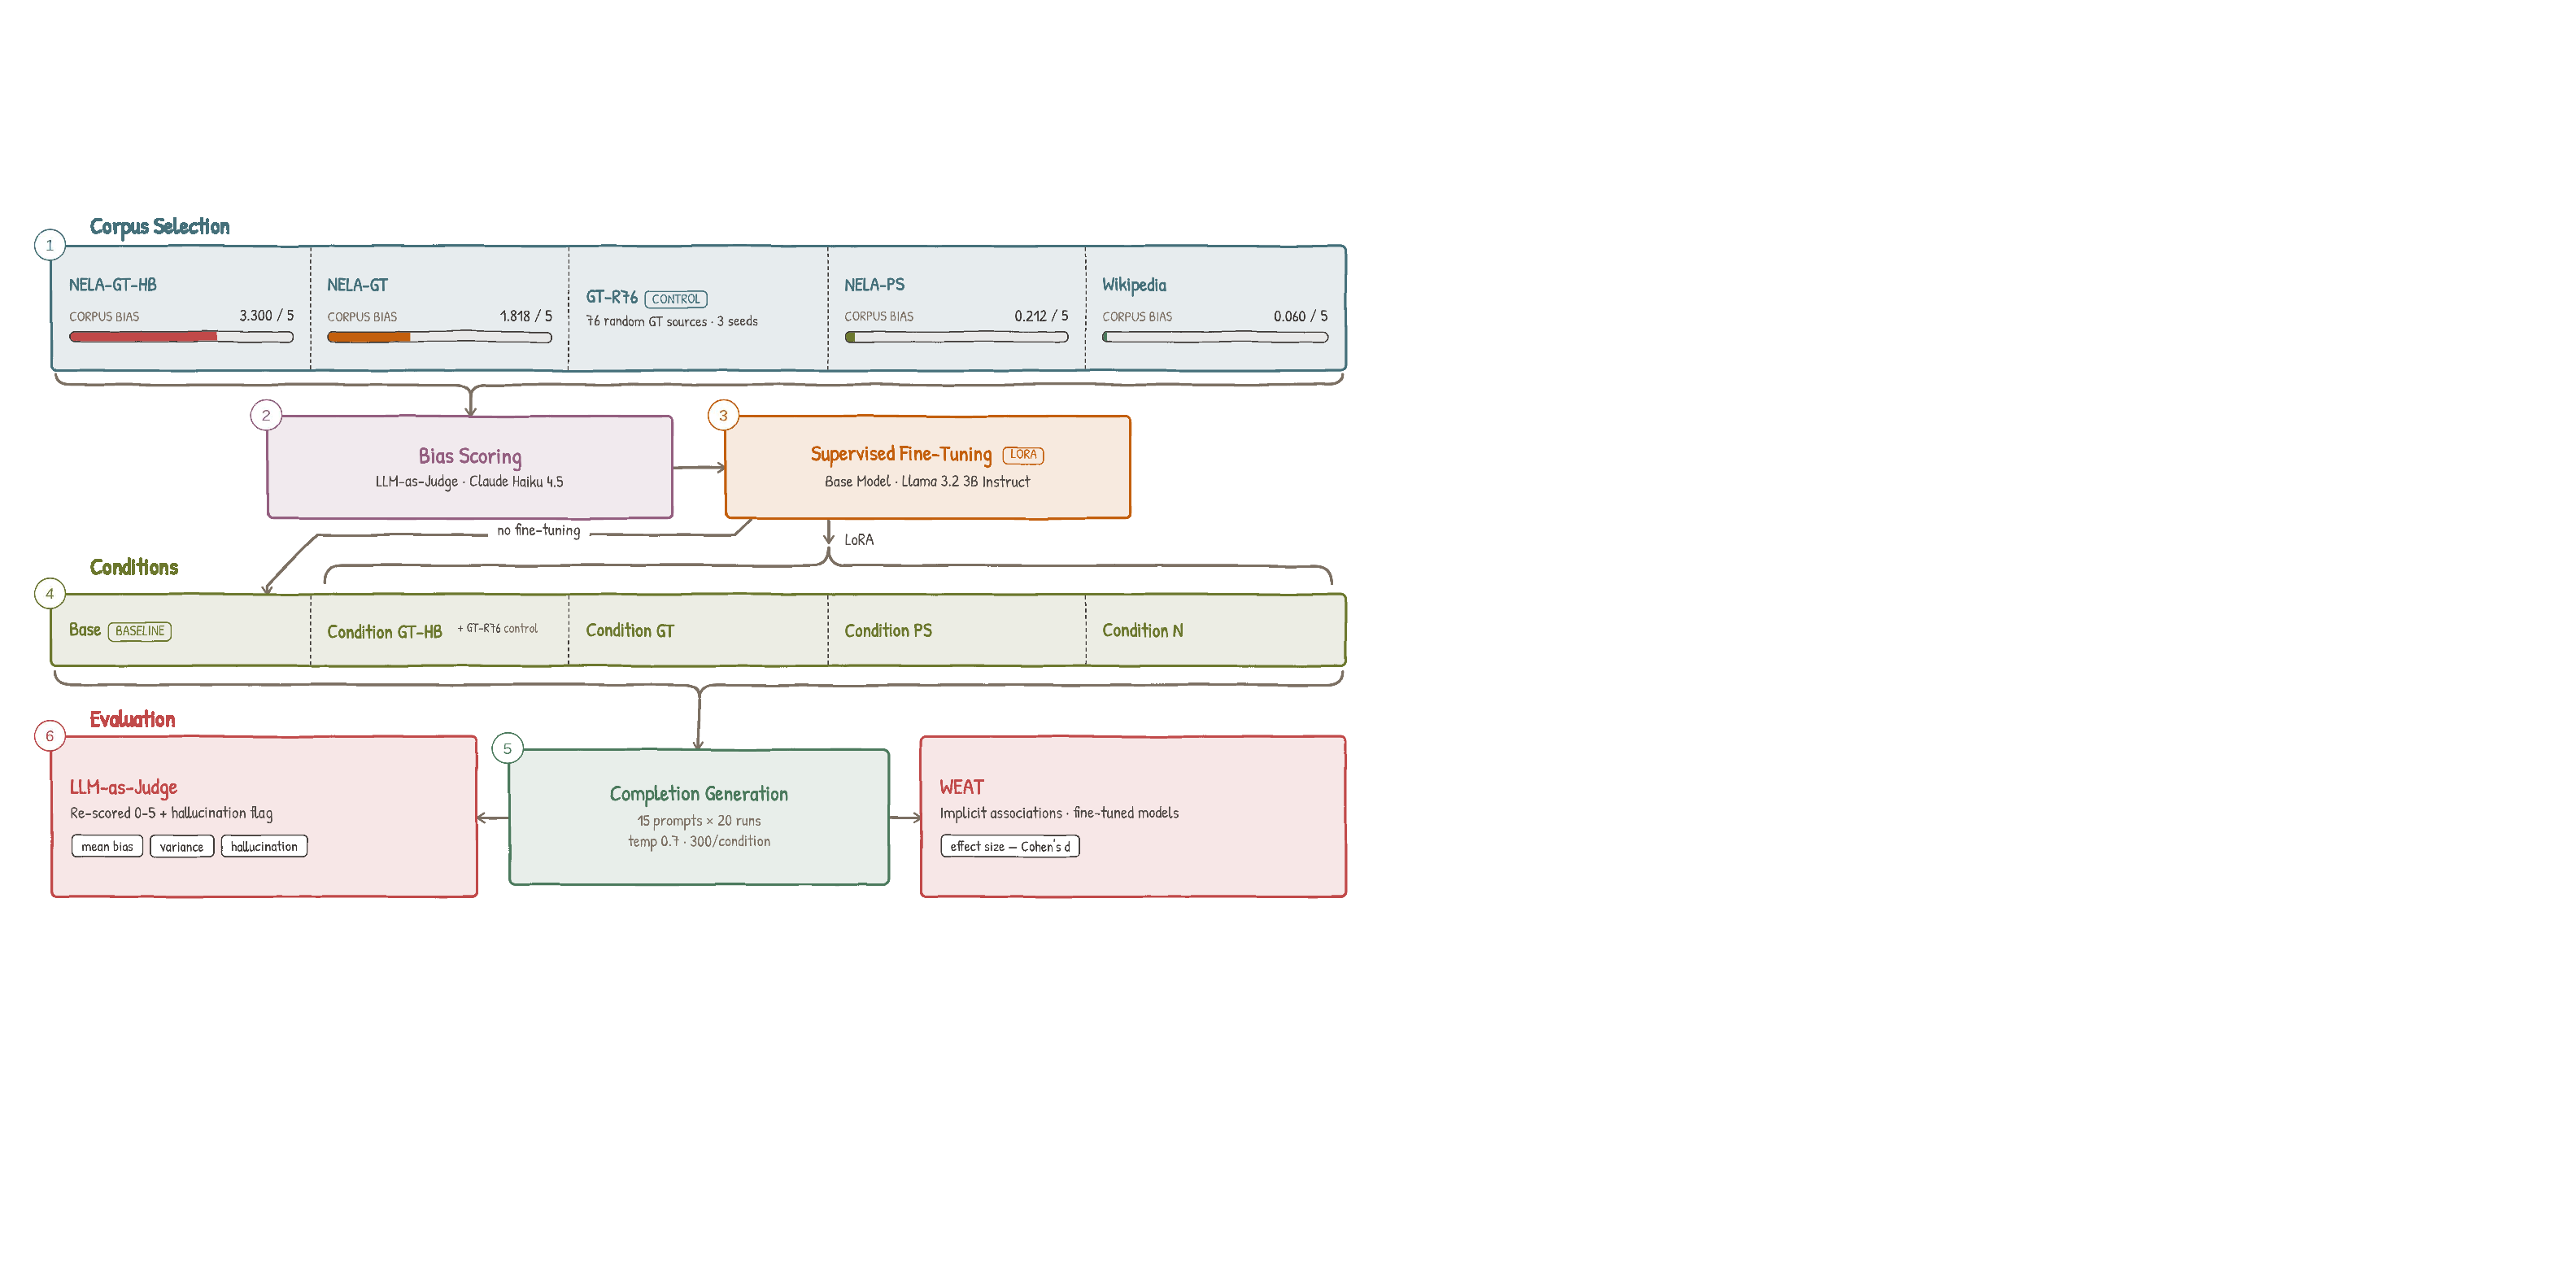
\includegraphics[width=\gridwidth,trim=1.5 1.5 1.0 0,clip]{../plots/pipeline-latest-short.pdf}}
{\centering\tabcaption{Pipeline overview: from corpus selection and fine-tuning through completion generation to dual evaluation by LLM-as-Judge and WEAT. Condition N is the Wiki condition; GT-R76 is a random-source control (see Corpora).}}
\vskip 0.4cm

\begin{columns}[t]

% ===================================================================
\begin{column}{0.315\paperwidth}

\begin{block}{1. Question \& Setup}
  \key{We examine how a training corpus's bias transfers to a model fine-tuned on it.}
  \begin{itemize}
    \item \textbf{Model:} Llama 3.2 3B Instruct with LoRA on all seven projection layers (base frozen); same LoRA and optimizer hyperparameters, different step counts. Unmodified $=$ Base.
    \item \textbf{Four corpora spanning a bias range:} partisan NELA-GT news, its high-bias filtered subset NELA-GT-HB (76 sources with source-mean bias $\ge 3$), auto-generated NELA-PS pink-slime content, and Wikipedia articles on US high schools (Wiki).
    \item \textbf{Completions:} 15 prompts (education, immigration, climate, policing, \ldots) $\times$ 20 runs $=$ 300 per condition, \key{1{,}500 total}; 150 tokens, temperature 0.7.
    \item \textbf{Bias scoring:} LLM-as-Judge (Claude Haiku 4.5, 0--5 rubric: 0 purely factual $\to$ 5 propaganda) on every completion, and WEAT on last-layer embeddings.
    \item \textbf{Significance:} prompt-level one-sided Wilcoxon signed-rank vs.\ Base, Holm-corrected; 95\% CIs by bootstrap over prompts.
  \end{itemize}
\end{block}

\begin{block}{2. Corpora}
  \centering
  \small
  \setlength{\tabcolsep}{0.42em}
  \begin{tabular}{lrrrcr}
    \toprule
    Corpus & Samples & Steps & Final Loss & Bias Mean & \% Bias $= 0$ \\
    \midrule
    NELA-GT     & 500{,}000 & 5{,}000  & 1.855 & 1.818 & 28.8 \\
    NELA-GT-HB  & 500{,}000 & 5{,}000  & 1.917 & 3.300 &  0.8 \\
    NELA-PS     & 500{,}000 & 5{,}000  & 0.572 & 0.212 & 94.4 \\
    Wiki        & 10{,}000  & 15{,}625 & \textbf{0.032} & 0.060 & 96.2 \\
    \bottomrule
  \end{tabular}
  \tabcaption{Corpus bias: mean judge score and \% of a 500-article sample scoring 0. Final loss after fine-tuning.}
  \normalsize
  \vskip 0.6ex
  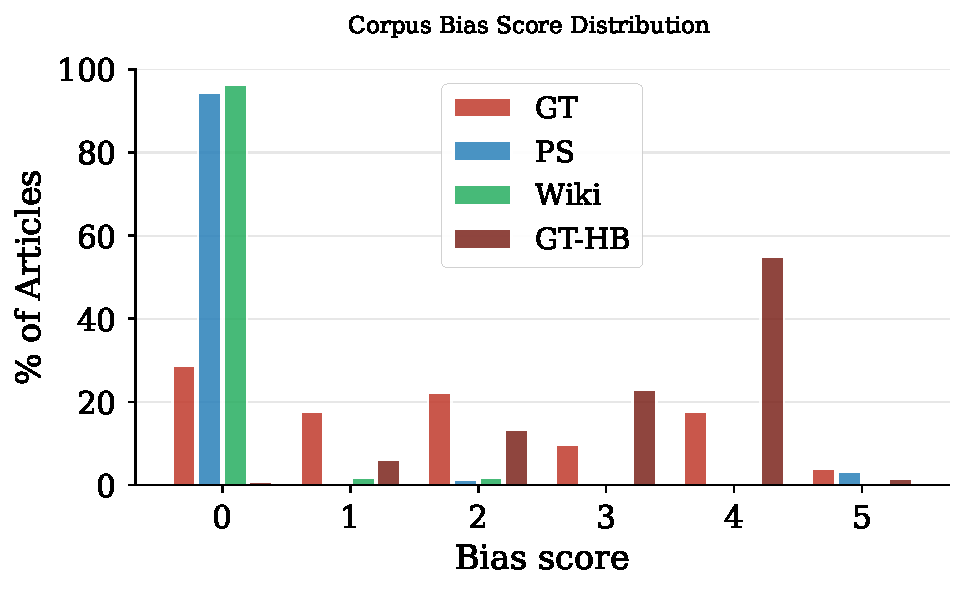
\includegraphics[width=0.68\linewidth]{corpus_distribution_poster.pdf}
  \tabcaption{Distribution of bias scores (0--5) across the four training corpora.}
  \raggedright
  \begin{itemize}
    \item A held-out 500-article re-score confirms GT-HB's filtering: 93.0\% of articles have bias $\ge 2$, vs.\ GT's 53.6\%.
    \item Control GT-R76 (76 random NELA-GT sources, 3 seeds) averages 1.485, close to GT's 1.470 and well below GT-HB's 1.763: GT-HB's effect is source bias, not concentration.
  \end{itemize}
\end{block}

\begin{block}{Limitations}
  \begin{itemize}
    \item Wiki trained 15{,}625 steps on 10{,}000 articles (vs.\ 5{,}000 on 500{,}000) and memorized its corpus.
    \item Single judge (Claude Haiku 4.5); a second judge (Qwen3.5-27B) agrees on relative ordering (Spearman $\rho=0.90$) but not absolute scores.
    \item Single model, temperature 0.7; on the 3 significant prompts, GT $>$ Base $>$ PS holds at 0.3 and 1.0.
  \end{itemize}
\end{block}

\end{column}

% ===================================================================
\begin{column}{0.315\paperwidth}

\begin{block}{3. Output bias (LLM-as-Judge)}
  \centering
  \small
  \setlength{\tabcolsep}{0.35em}
  \begin{tabular}{lcccccccc}
    \toprule
    Condition & Mean & \%$_{0}$ & \%$_{1}$ & \%$_{2}$ & \%$_{3}$ & \%$_{4}$ & \%$_{5}$ & $p_{\text{Holm}}$ \\
    \midrule
    Base      & 0.847 & 23.3 & 68.7 &  8.0 &  0.0 &  0.0 &  0.0 & --     \\
    GT        & 1.470 & 24.0 & 19.3 & 46.7 &  7.0 &  1.7 &  1.3 & 0.0015 \\
    GT-HB     & 1.763 & 20.0 & 15.3 & 43.3 & 12.0 &  8.3 &  1.0 & 0.0015 \\
    PS        & 0.507 & 69.0 & 16.3 & 11.3 &  2.0 &  1.0 &  0.3 & 0.0015 \\
    Wiki      & \textbf{2.153} & 13.3 & 20.7 & 35.3 &  8.3 & 12.7 &  9.7 & 0.0013 \\
    \bottomrule
  \end{tabular}
  \tabcaption{Output bias scores across all 15 prompt topics ($n = 300$ per condition). $p_{\text{Holm}}$: Holm-adjusted one-sided Wilcoxon signed-rank $p$-value against Base, on prompt-level means.}
  \normalsize
  \raggedright
  \begin{itemize}
    \item \key{All four bias shifts are significant.} Mean differences with 95\% CIs: GT $+0.623$ $[0.457, 0.800]$; GT-HB $+0.917$ $[0.650, 1.163]$; Wiki $+1.307$ $[0.843, 1.820]$; PS $-0.340$ $[-0.460, -0.220]$. No interval crosses zero.
    \item GT exceeds Base unevenly: climate ($\mu=2.350$) and immigration ($\mu=2.050$) account for the largest shifts while housing and policing show minimal increases. PS reduces bias below Base.
    \item GT-HB's mean exceeds GT's on 13 of 15 topics, yet gains are near-zero where GT already peaked (climate $+0.05$) and largest on topics GT left largely unaffected (education $+1.00$, tech regulation $+1.00$): a \key{broadening} of bias, suggesting a saturation limit.
  \end{itemize}
\end{block}

\begin{block}{4. WEAT associations}
  \centering
  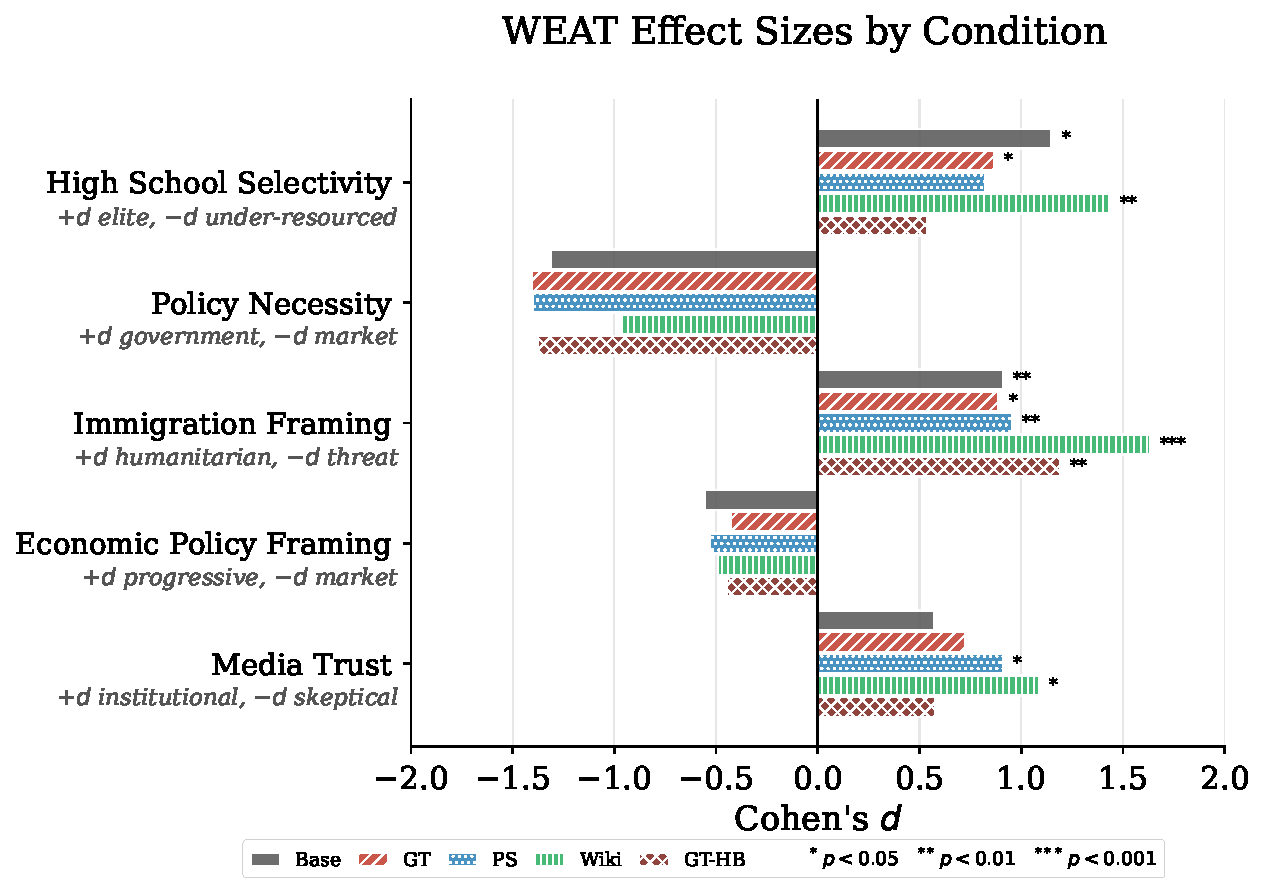
\includegraphics[width=\linewidth]{weat_effects_poster.pdf}
  \tabcaption{WEAT effect sizes (Cohen's $d$) by condition and test, with significance markers from the one-sided permutation test. Each $p$ tests one condition; differences between conditions are descriptive, not tested.}
  \raggedright
  \begin{itemize}
    \item Test 3 (Immigration Framing) produces the experiment's largest effect size: \key{Wiki, $d = +1.632$, $p < 0.001$}, a strong association between humanitarian immigration framing and positive attributes; Wiki also has the highest immigration bias rate ($100\%$) and mean ($4.05$).
    \item GT-HB's humanitarian association ($d = +1.190$, $p = 0.001$) is larger than Base's, GT's, and PS's ($+0.911$, $+0.890$, $+0.955$), with a hallucination rate of only $12.0\%$: genuine framing amplification rather than fabrication.
    \item Tests 2 and 4 show associations opposite to the hypothesized direction in every condition (Test 2: $d$ from $-0.97$ to $-1.41$; Test 4: $d$ from $-0.43$ to $-0.56$).
  \end{itemize}
\end{block}

\end{column}

% ===================================================================
\begin{column}{0.315\paperwidth}

\begin{alertblock}{5. The Wiki Paradox}
  Despite the lowest corpus bias, Wiki has the highest raw output bias and largest WEAT effects, and is the only condition that hallucinates abnormally (e.g.\ a nonexistent ``Migrant Children's Rights Act of 2022'').
  \vskip 0.6ex
  \centering
  \small
  \setlength{\tabcolsep}{0.45em}
  \begin{tabular}{lrrrrr}
    \toprule
    Condition & Hall. Rate & Corr. Rate & $\mu_{all}$ & $\mu_{clean}$ & $\Delta\mu_{hall.}$ \\
    \midrule
    Base      & 2.0\%      & --         & 0.847       & --            & --                  \\
    GT        & 10.7\%     & 2.1\%      & 1.470       & 1.439         & +0.031              \\
    PS        & 5.3\%      & --         & 0.507       & --            & --                  \\
    Wiki      & \textbf{44.3\%}     & \textbf{36.9\%}     & 2.153       & 1.484         & \textbf{+0.669}              \\
    GT-HB     & 12.0\%     & 4.8\%      & 1.763       & 1.686         & +0.077              \\
    \bottomrule
  \end{tabular}
  \tabcaption{Hallucination rate and precision-corrected bias score per condition. Corr. Rate and $\mu_{clean}$ correct for the flag's false-positive rate; $\Delta\mu_{hall.}$ is the reduction from $\mu_{all}$ to $\mu_{clean}$. Shown only for conditions with validated flag precision.}
  \normalsize
  \vskip 0.6ex
  \begin{beamercolorbox}[wd=\linewidth,sep=0.6em]{block title}
    \centering\large\bfseries
    After false-positive correction, 36.9\% of Wiki's completions include fabricated laws, policies, or officials\\[0.4ex]
    Across prompts, Wiki's bias score tracks its hallucination rate: $r = 0.94$
  \end{beamercolorbox}
  \vskip 0.6ex
  \raggedright
  Three possible, non-exclusive explanations:
  \begin{enumerate}
    \item \key{Overfitting with excess training steps.} 50 epochs over 10{,}000 articles (15{,}625 steps); final loss 0.032 indicates near complete memorization.
    \item \key{Hallucination-driven score inflation.} The judge flags hallucination in 44.3\% of Wiki's completions, including every Climate and Immigration completion. Correcting for the flag's false-positive rate, its mean drops from 2.153 to 1.484 (31\%); the other validated conditions (GT, GT-HB) move by at most 0.077. Whether Wiki ranks above or below GT-HB after correction depends on topic weighting (pooled 1.484 vs.\ 1.686; equal-weighted 1.860 vs.\ 1.693).
    \item \key{Amplification of pre-existing bias.} Wikipedia's own skews (domain coverage, editor demographics) plausibly shape inherited associations that fine-tuning intensifies. Most defensibly these interact: overfitting amplifies a weak immigration signal, and the base model's pro-immigration association ($d = +0.911$) supplies the fake legislative content.
  \end{enumerate}
\end{alertblock}

\begin{block}{6. Takeaways}
  \begin{itemize}
    \item Partisan news (GT) transferred bias on specific topics; the most biased sources (GT-HB) strengthen and broaden it, surviving hallucination cleaning (1.686 $>$ 1.439); near-neutral PS reduced bias.
    \item \key{For Llama 3.2 3B Instruct under our fine-tuning setup, corpus-level bias scores are not reliable predictors of fine-tuned model bias.} Corpora that appear neutral on the surface can still produce fine-tuned models with high bias scores when training develops into memorization.
    \item \key{In the same setup, LLM-as-Judge evaluations of bias risk conflating factual accuracy with actual bias in models that hallucinate more.}
  \end{itemize}
\end{block}

\end{column}
\end{columns}
\end{frame}
\end{document}
